\documentclass[12pt]{article}
\newcommand\tab[1][1cm]{\hspace*{#1}}
\usepackage{amsmath,amssymb,amsthm}
\usepackage{graphicx,mathabx}
\usepackage{xcolor}
\usepackage{mathabx}
\usepackage{tikz}
\usepackage{cases}
\usepackage{placeins}
\usepackage{lipsum}
\usepackage{multirow}
\usepackage{mathtools}
\usepackage[shortlabels]{enumitem}
\usepackage{wrapfig}
\DeclarePairedDelimiter{\floor}{\lfloor}{\rfloor}
\begin{document}
\title{TCSS 343 - Week 7 - Monday}
\author{Jake McKenzie}
\maketitle
\noindent\centerline{\textbf{More Dynamic Programming and varied Shortest Path Problems}}\\\\\\\\\\\\
\begin{center}
    ``People say nothing is impossible, but I do nothing every day." \\$\cdots$\\ Winnie the Poo
\end{center}
\begin{center}
    ``It is not enough to be in the right place at the right time. You should also have an open mind at the right time." \\$\cdots$\\ Paul Erd\H{o}s
\end{center}
\begin{center}
    ``Nothing in life is to be feared, it is only to be understood. Now is the time to understand more, 
    so that we may fear less." \\$\cdots$\\ Marie Curie
\end{center}
\newpage
\begin{enumerate}
\item[0.] What are the two characteristics of a dynamic programming problem? (What kind of substructures and subproblems do you have?)\\\\\\\\\\\\\\\\
\item Is merge sort a candidate for dynamic programming? Why or why not? 
\newpage
\item Given a string $S=\text{ABAZDC}$ and $T=\text{BACBAD}$ compute the longest common subsequence between the two strings. For your convenience:\\
\[
L(i,j) = \left\{
\begin{tabular}{cc}
0 & \text{if} $i = 0 \lor j = 0$ \\
L[i-1,j-1] + 1 & \text{if} $i > 0, j > 0 \land a_i = b_j$  \\
max\{L[i,j-1],L[i-1,j]\} & \text{if} $i > 0, j > 0 \land a_i \ne b_j$   \\
\end{tabular}\right.
\]
\newpage
\item Look back to your notes from lecture for the knapsack problem. Imagine you have a homework assignment 
with different segments labeled A through G. Each part has a ``value" (in points) and a ``size" (time in hours to complete). 
For example, say the values and times for our assignment are: \\
\centerline{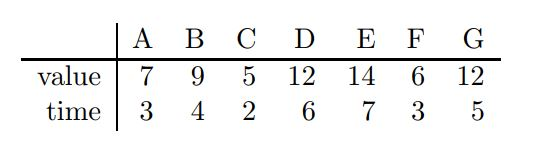
\includegraphics[scale = 0.8]{ks.jpg}}\\
Say you have a total of 15 hours: which parts should you do? If there was partial credit that was
proportional to the amount of work done (e.g., one hour spent on problem C earns you 2.5 points)
then the best approach is to work on problems in order of points/hour (a greedy strategy). But,
what if there is no partial credit? In that case, which parts should you do, and what is the best
total value possible?
\newpage
\item Let us say we have a set of rectangular blocks $\{1,2,\dots , n\}$, where each block has a length $l_i$,
a width $w_i$, and height $h_i$. You want to stack blocks to get the maximum height. In order to stack block $j$ on top of 
block $i$ you require $l_j < l_i$ $\land$ $w_j < w_i$. Also there is a single orientation allowed for each block, where each 
side has a fixed north, south, east and west.  Finish the reduction below:\\
$$RB(1,2,\dots , n) = \max_i\{h_i + RB(\tab[5cm])\}$$
\\\\\\\\\\\\\\\\\\\\
\item Let us now analyze the runtime. The first question you should always ask: How many subproblems do we have? Use the reduction to help you 
find what subproblems there are for this problem.
\newpage
\item Consider the following undirected, weighted graph:\\
\centerline{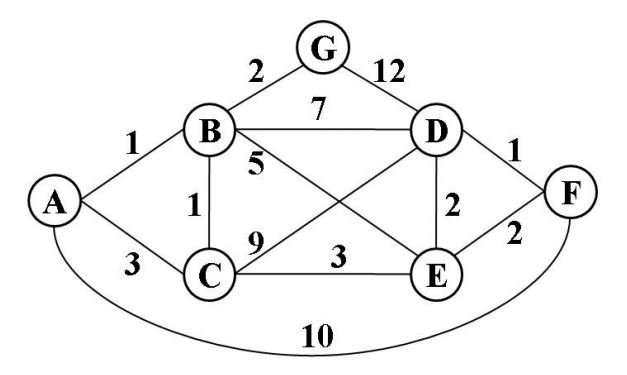
\includegraphics[scale = .7]{graph.jpg}}\\
Step through Dijkstra’s algorithm to calculate the single-source shortest 
paths from A to every other vertex. Show your steps in the table below. 
Cross out old values and write in new ones, from left to right within each 
cell, as the algorithm proceeds. Also list the vertices in the order which 
you marked them known. Finally, indicate the lowest-cast path from node A 
to node F.\\
\textbf{Known vertices:} $\rule{1cm}{0.15mm}$ $\rule{1cm}{0.15mm}$ $\rule{1cm}{0.15mm}$ $\rule{1cm}{0.15mm}$ $\rule{1cm}{0.15mm}$ $\rule{1cm}{0.15mm}$ $\rule{1cm}{0.15mm}$\\
\textbf{(in order marked known)}\\
\centerline{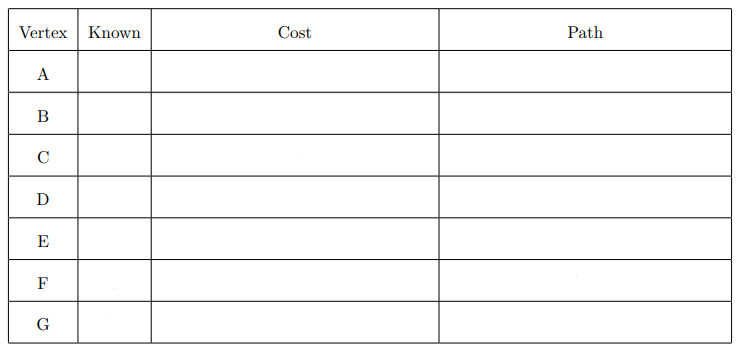
\includegraphics[scale = 2]{table.jpg}}\\\\
\textbf{Lowest-cost path from A to F:} $\rule{7cm}{0.15mm}$
\newpage 
\item Consider the following directed, weighted graph:\\
\centerline{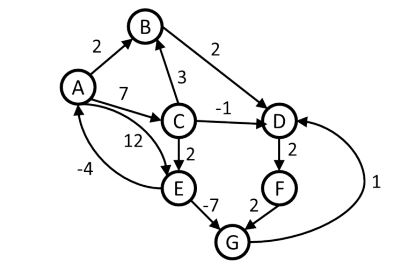
\includegraphics[scale = 0.7]{graph3.jpg}}\\
Even though the graph has negative weight edges, step through Dijkstra’s algorithm to calculate
\textit{supposedly} shortest paths from A to every other vertex. Show your steps in the table below.
Cross out old values and write in new ones, from left to right within each cell, as the algorithm
proceeds. Also list the vertices in the order which you marked them known.
Dijkstra’s algorithm found the wrong path to some of the vertices. For just the vertices where
the wrong path was computed, indicate both the path that was computed and the correct path.\\\\
\textbf{Known vertices:} $\rule{1cm}{0.15mm}$ $\rule{1cm}{0.15mm}$ $\rule{1cm}{0.15mm}$ $\rule{1cm}{0.15mm}$ $\rule{1cm}{0.15mm}$ $\rule{1cm}{0.15mm}$ $\rule{1cm}{0.15mm}$\\
\textbf{(in order marked known)}\\
\centerline{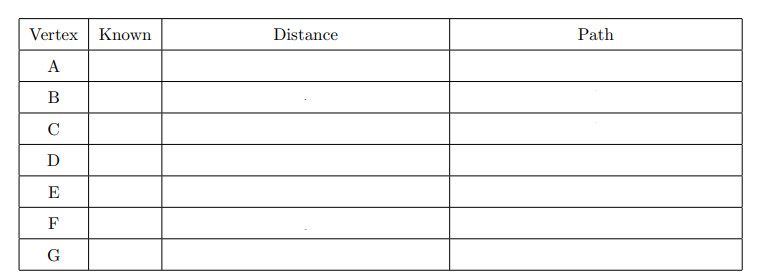
\includegraphics[scale = 1.75]{table2.jpg}}\\
\item What single edge could be removed from the graph such that Dijkstra’s algorithm would happen
to compute correct answers for all vertices in the remaining graph?
\end{enumerate}
\end{document}